\textbf{Входные параметры:}
 
Data --- данные о нечетких числах
 
[0] --- a1, левая крайняя граница первого нечеткого трапециевидного числа.
 
[1] --- b1, начало устойчивой области первого нечеткого трапециевидного числа.
 
[2] --- с1, конец устойчивой области первого нечеткого трапециевидного числа.
 
[3] --- d1, правая крайняя граница первого нечеткого трапециевидного числа.
 
[4] --- a2, левая крайняя граница второго нечеткого трапециевидного числа.
 
[5] --- b2, начало устойчивой области второго нечеткого трапециевидного числа.
 
[6] --- с2, конец устойчивой области второго нечеткого трапециевидного числа.
 
[7] --- d2, правая крайняя граница второго нечеткого трапециевидного числа.

\textbf{Возвращаемое значение:}
 
Максимальное значение функции принадлежности нечеткого числа.

 \begin{figure} [h] 
   \center
   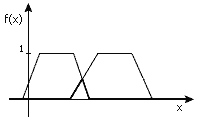
\includegraphics {HML_MaxiMinTrapeziformFuzzyNumbers.png}
   \caption{График:} 
   \label{img:HML_MaxiMinTrapeziformFuzzyNumbers}  
 \end{figure}